
\PassOptionsToPackage{colorlinks,linkcolor={blue},citecolor={blue},urlcolor={blue},breaklinks=true,final}{hyperref}
\PassOptionsToPackage{dvipsnames}{xcolor}
\documentclass[xcolor={dvipsnames,svgnames},aspectratio=169]{beamer}

\usepackage{fontawesome5}
\usepackage{booktabs} % For better table formatting
\usepackage{listings}
\usepackage{tabularx}


\lstset{
  tabsize = 4, %% set tab space width
  showstringspaces = false, %% prevent space marking in strings, string is defined as the text that is generally printed directly to the console
  numbers = left, %% display line numbers on the left
  commentstyle = \color{purple!60}, %% set comment color
  keywordstyle = \color{blue}, %% set keyword color
  stringstyle = \color{red}, %% set string color
  rulecolor = \color{black}, %% set frame color to avoid being affected by text color
  basicstyle = \small \ttfamily , %% set listing font and size
  breaklines = true, %% enable line breaking
  numberstyle = \tiny,
}

\title{Concurrent Programming}
\subtitle{Week 13 (Lecture 6)}
\author{Stelios Tsampas}
\institute{
  \faEnvelope \; stelios@imada.sdu.dk
  \qquad
  \faGlobe \;
  \href{https://www.steliostsampas.com}{https://www.steliostsampas.com}
  \\\\\
  \faGithub \; stelios-tau/cp-2025
  \qquad\;\;
    \faDiscord \; cp-2025
}
\date{\today}

\titlegraphic{\includegraphics[height=0.6cm,keepaspectratio]{../media/sdu-black.eps}}

\usetheme[block=fill]{metropolis}


%\usepackage{pres-common}
\usepackage{textpos}
\usepackage{centernot}

% \newcommand{\Goesv}[3]{\ensuremath{#1 \xRightarrow{~#3~} #2}}
% \newcommand{\goesv}[3]{\ensuremath{#1 \xrightarrow{~#3~} #2}}

% \usepackage{etex}
% \usepackage{semantic}

\usepackage[utf8]{inputenc}
\usepackage[english]{babel}
\usepackage{tikz}
\usepackage{hyperref}

\usetikzlibrary{arrows,shapes,matrix}
\usetikzlibrary{backgrounds}
\usetikzlibrary{positioning}
\usetikzlibrary{automata}
\usetikzlibrary{mindmap}
\usetikzlibrary{shapes.callouts}
\usetikzlibrary{decorations.text}
\usetikzlibrary{tikzmark}
\usetikzlibrary{calc}
\usetikzlibrary{overlay-beamer-styles}
\usetikzlibrary{shapes.geometric}
\usepackage{pgfplots}


\tikzset{onslide/.code args={<#1>#2}{%
    \only<#1>{\pgfkeysalso{#2}} % \pgfkeysalso doesn't change the path
  }}

\setbeamercolor{mygray}{bg=Gray!20}

\tikzset{temporal/.code args={<#1>#2#3#4}{%
    \temporal<#1>{\pgfkeysalso{#2}}{\pgfkeysalso{#3}}{\pgfkeysalso{#4}} % \pgfkeysalso doesn't change the path
  }}

\tikzstyle{highlight}=[fill=green!50]
\tikzstyle{hgreen}=[fill=green!20]
\tikzstyle{hred}=[fill=red!50]
\tikzstyle{hblue}=[fill=blue!50]
\tikzstyle{hgray}=[fill=gray!50]

\addtobeamertemplate{frametitle}{}{%
\begin{textblock*}{100mm}(\textwidth-2cm,-0.86cm)
\includegraphics[height=0.6cm,keepaspectratio]{../media/sdu-white.eps}
\end{textblock*}}


%\usepackage{tikz-cd}
% \usepackage{wasysym}
% \usepackage{color}
% \usepackage[matrix,arrow]{xy}
% \xyoption{all}
% \SelectTips{cm}{}
% % \usepackage{cite}
% \usepackage{amsthm}
% \usepackage{amsmath}
% \usepackage{bbold}
% % \usepackage[bbgreekl]{mathbbol}
% \usepackage{amssymb}
% \usepackage{pifont}
% \usepackage{mathtools}
% \usepackage{amsbsy}
% % \usepackage{paralist}
% \usepackage{shadethm}
% % \usepackage{fancyhdr}
% \usepackage{stmaryrd}
% \usepackage{wasysym}
% \usepackage{graphicx}
% \usepackage{tabularx}
% \usepackage{dsfont}
% \usepackage{ulem}




%\bibliography{mainBiblio}

%\includeonlyframes{current}
\begin{document}

\frame{\titlepage}

\def\firstcircle{(0,0) circle (2cm)}
\def\secondcircle{(1.4,1.4) circle (2cm)}
\def\thirdcircle{(0:2.4) circle (2cm)}

\begin{frame}{Outline}
  \tableofcontents
\end{frame}

\section{Recap}

\begin{frame}[fragile]
  \frametitle{Last week's topics}

  Last lecture, we touched upon...

  \begin{itemize}
  \item[\faBook]<1-> How to design software that can be
    \emph{utilized} safely in a concurrent setting.
  \item[\faBook]<1-> \emph{Visibility} in all its weirdness.
  \item[\faBook]<1-> The tricky topic of object \emph{sharing}.
  \item[\faBook]<1-> The role of \emph{invariants}, \emph{immutability} and
    \emph{encapsulation}.
  \end{itemize}
\end{frame}

\begin{frame}[fragile]
  \frametitle{Some lessons so far}

  \begin{block}{\faBook\quad It's all about the mutable state.}
    All concurrency issues boil down to coordinating access to mutable
    state. The less mutable state, the easier it is to ensure thread safety.
  \end{block}

  \vspace{0.2cm}

  \begin{block}<2->{\faBook\quad Immutable objects are thread-safe.}
    Immutable objects simplify concurrent programming tremendously.
    They are simpler and safer, and can be shared freely without locking
    or defensive copying.
  \end{block}

  \vspace{0.2cm}

  \begin{block}<3->{\faBook\quad Encapsulation simplifies concurrency.}
    Organizes mutable states, hence organizes the invariants and makes them more
    manageable.
  \end{block}
\end{frame}

\begin{frame}[fragile]
  \frametitle{Some lessons so far (cont.)}

  \begin{itemize}
  \item[\faBook]<1-> If a field is not mutable, make it \textbf{final}.
  \item[\faBook]<1-> Guard each mutable variable with a \textbf{lock}.
  \item[\faBook]<1-> Guard all variables in an \textbf{invariant} with the
    \textbf{same} lock.
  \item[\faBook]<1-> Hold locks for the duration of compound actions.
  \item[\faBook]<1-> Don’t rely on visibility, obscure knowledge of the memory
    model or generally clever reasoning instead of synchronizing.
  \item[\faBook]<1-> Make thread safety a \textbf{central part} of your design
    process.
  \end{itemize}
\end{frame}

\begin{frame}[fragile]
  \frametitle{Learning flow}

  \begin{itemize}
  \item[\faBook]<1-> At this point, we are going to stop strictly following the book's
    structure (like we have been doing). The lectures are going to center more
    around the Plans (and their videos) themselves.
  \end{itemize}
\end{frame}

\begin{frame}[fragile]
  \frametitle{This week's topics}

  This week, we will look at...

  \begin{itemize}
  \item[\faBook]<1-> Spinlocks!
  \item[\faBook]<1-> Latches!
  \item[\faBook]<1-> Concurrent Collections!
  \end{itemize}

  \begin{itemize}
  \item[\faUserInjured]<2-> We will also demonstrate all of the above in
    examples.
  \end{itemize}
\end{frame}

\section{Spinlocks}

\begin{frame}[fragile]
  \frametitle{Why spin?}

  \begin{columns}
    \begin{column}{0.5\textwidth}
      \begin{itemize}
      \item<1->[\faBook] It is a pattern (busy-wait) that a beginner coder could
        come up with.
      \item<2->[\faBook] Often not the best choice\dots
      \item<3->[\faBook] But situationally it makes sense!
      \end{itemize}

      \vspace{1cm}

      \begin{itemize}
      \item<4->[\faSearch] Basically the Garen of concurrency.
      \end{itemize}
    \end{column}
    \begin{column}{0.5\textwidth}  %%<--- here
      \uncover<4->{
      \begin{center}
        \includegraphics[height=7cm,keepaspectratio]{../media/garen.jpg}
      \end{center}}
    \end{column}
  \end{columns}
\end{frame}

% \begin{frame}[fragile]
%   \begin{center}
%     \begin{figure}
%       \includegraphics[height=7cm,keepaspectratio]{../media/Steve.png}
%       \caption{A perhaps accurate depiction of the earlier phenomenon.}
%     \end{figure}
%   \end{center}
% \end{frame}

\begin{frame}[fragile]
  \frametitle{What are spinlocks}

  \begin{block}{\faLock\quad Spinlock}
    A type of lock where a thread repeatedly checks if the lock is available.
  \end{block}

  \begin{itemize}
  \item[\faBook]<1-> A thread busy-waits in a loop ("spins") instead of sleeping.
  \item[\faBook]<1-> Example of a non-blocking synchronization primitive.
  \item[\faBook]<1-> Used when:
    \begin{itemize}
    \item[\faCheck] Critical section is very short.
    \item[\faCheck] Threads are expected to wait only briefly.
    \end{itemize}
  \end{itemize}

  \begin{block}<2->{\faLightbulb \quad Key idea}
    Avoid the overhead of OS thread context switches: the spinning thread will
    not get suspended immediately if it fails to acquire the lock. This is
    potentially good for performance, as suspending and resuming threads is
    expensive.
  \end{block}
\end{frame}

\begin{frame}[fragile]
  \frametitle{Busy-wait}

\begin{lstlisting}[language = Java , frame = trBL , firstnumber = last ,
escapeinside={(*@}{@*)}]
while ((something) == 0) {
        /* do nothing - just keep checking over and over */
    }

doSomething();
\end{lstlisting}

  \vspace{0.2cm}
  \begin{block}<1->{\faLightbulb \quad Key idea}
    Wait -- and keep checking -- until a condition is met.
  \end{block}
\end{frame}

\begin{frame}[fragile]
  \frametitle{Spinlocks in Java}

\begin{lstlisting}[language = Java , frame = trBL , firstnumber = last ,
escapeinside={(*@}{@*)}]
import java.util.concurrent.atomic.AtomicBoolean;
[...]
private final AtomicBoolean locked = new AtomicBoolean(false);
[...]
    while (!locked.compareAndSet(false, true)) {
            Thread.onSpinWait(); // Optional hint (Java 9+)
        }
    doSomething(;)
    locked.set(false);
[...]
\end{lstlisting}

  \begin{block}<1->{\faLightbulb \quad \texttt{compareAndSet}'s role}
  Sets \texttt{locked} to \texttt{true} if it is \texttt{false} (atomically).
  Returns \texttt{false} otherwise.
  \end{block}
\end{frame}

\begin{frame}[fragile]
  \frametitle{Compare with \texttt{synchronized}}

\begin{lstlisting}[language = Java , frame = trBL , firstnumber = last ,
escapeinside={(*@}{@*)}]
private final Object lock = new Object();

public void doWorkWithSynchronizedLock() {
    synchronized (lock) {
        doSomething(); // critical section
    }
}
\end{lstlisting}

\end{frame}

\begin{frame}[fragile]
  \frametitle{Spinlock vs \texttt{synchronized} (Blocking)}
  \begin{table}[]
    \centering
    \begin{tabular}{l|l|l}
        \toprule
      \textbf{}
      & \textbf{Spinlock}
      & \textbf{Synchronized / Blocking Lock} \\
        \midrule
      \textbf{Behavior}
      & Active waiting (spins)
      & Passive waiting (thread blocks)\\
        \midrule
      \textbf{CPU Usage}
      & High during contention
      & Low (thread sleeps)\\
        \midrule
      \textbf{Context switch}
      & Avoided (keeps spinning)
      & Incurred (expensive) \\
        \midrule
      \textbf{Best for}
      & Low-contention, short tasks
      & Longer critical sections \\
        \bottomrule
    \end{tabular}
  \end{table}

  \begin{block}<2->{\faExclamationTriangle \quad Important}
    Spinlocks waste CPU if contention is high!
  \end{block}
\end{frame}

% Four million each
% Benchmark: SpinLock
% SpinLock   &  1 threads &  4000000 inc/thread & 23.90 ms \\
% SpinLock   &  2 threads &  4000000 inc/thread & 194.69 ms \\
% SpinLock   &  4 threads &  4000000 inc/thread & 804.36 ms \\
% SpinLock   &  8 threads &  4000000 inc/thread & 3058.44 ms \\
% SpinLock   & 16 threads &  4000000 inc/thread & 11280.23 ms \\

% spinlock without hint
% SpinLock   &  1 threads &  4000000 inc/thread & 23.79 ms \\
% SpinLock   &  2 threads &  4000000 inc/thread & 255.91 ms \\
% SpinLock   &  4 threads &  4000000 inc/thread & 821.17 ms \\
% SpinLock   &  8 threads &  4000000 inc/thread & 3142.18 ms \\
% SpinLock   & 16 threads &  4000000 inc/thread & 11278.40 ms \\

% Benchmark: synchronized
% synchronized &  1 threads &  4000000 inc/thread & 17.45 ms \\
% synchronized &  2 threads &  4000000 inc/thread & 130.45 ms \\
% synchronized &  4 threads &  4000000 inc/thread & 210.27 ms \\
% synchronized &  8 threads &  4000000 inc/thread & 351.00 ms \\
% synchronized & 16 threads &  4000000 inc/thread & 749.40 ms \\

% Benchmark: Nothing
% SpinLock   &  1 threads &  4000000 inc/thread & 8.28 ms \\
% SpinLock   &  2 threads &  4000000 inc/thread & 57.00 ms \\
% SpinLock   &  4 threads &  4000000 inc/thread & 126.49 ms \\
% SpinLock   &  8 threads &  4000000 inc/thread & 244.12 ms \\
% SpinLock   & 16 threads &  4000000 inc/thread & 486.06 ms \\



\begin{frame}[fragile]
  \frametitle{Spinlock vs \texttt{synchronized} (Blocking) vs nothing}

  \begin{center}
  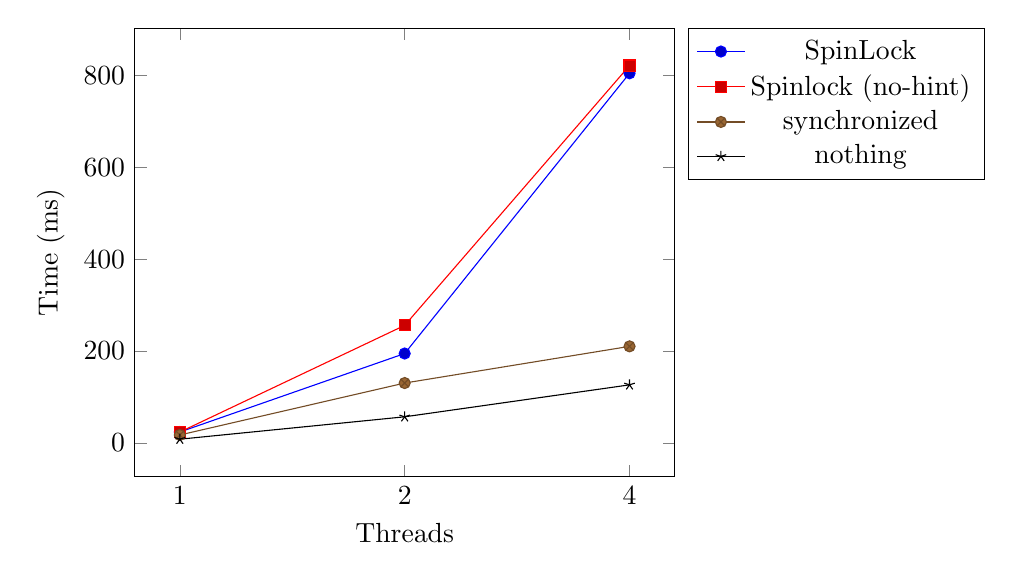
\begin{tikzpicture}
    \begin{axis}[
%      ybar,
      symbolic x coords={1,2,4,8,16},
      xtick=data,
      xlabel={Threads},
      ylabel={Time (ms)},
      legend style={at={(1.3,1)},anchor=north}
      ]
      \addplot coordinates {(1,23.90) (2,194.69) (4,804.36)};
      \addplot coordinates {(1,23.79) (2,255.91) (4,821.17)};
      \addplot coordinates {(1,17.45) (2,130.45) (4,210.27)};
      \addplot coordinates {(1,8.28) (2,57.00) (4,126.49)};
      \legend{SpinLock, Spinlock (no-hint),synchronized, nothing}
    \end{axis}
  \end{tikzpicture}
  \end{center}
\end{frame}

\begin{frame}[fragile]
  \frametitle{Spinlock vs \texttt{synchronized} (Blocking) vs nothing (cont.)}

  \begin{center}
  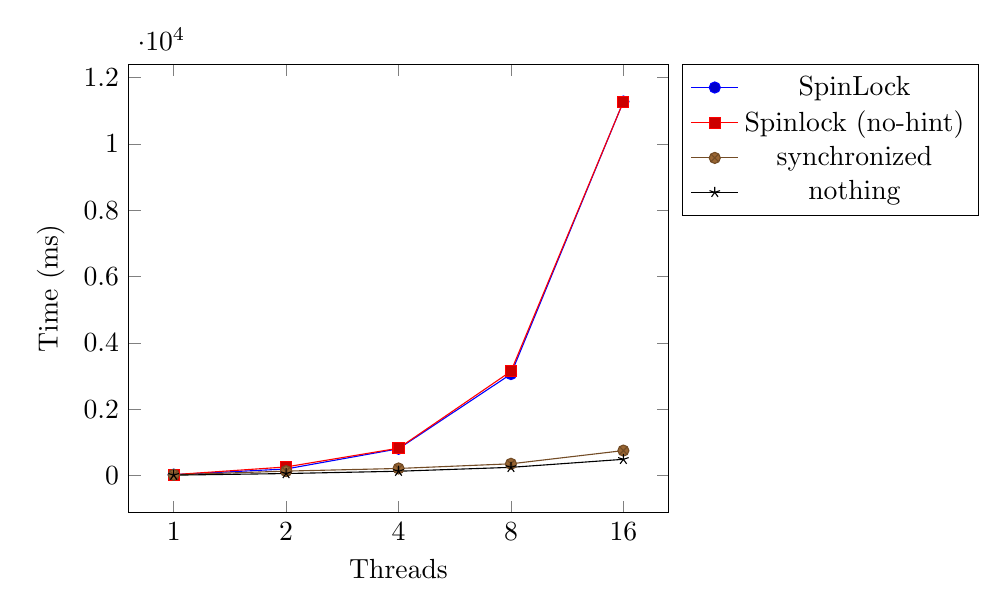
\begin{tikzpicture}
    \begin{axis}[
%      ybar,
      symbolic x coords={1,2,4,8,16},
      xtick=data,
      xlabel={Threads},
      ylabel={Time (ms)},
      legend style={at={(1.3,1)},anchor=north}
      ]
      \addplot coordinates {(1,23.90) (2,194.69) (4,804.36) (8,3058.44) (16,11280.23)};
      \addplot coordinates {(1,23.79) (2,255.91) (4,821.17) (8,3142.18) (16,11278.40)};
      \addplot coordinates {(1,17.45) (2,130.45) (4,210.27) (8,351.00) (16,749.40)};
      \addplot coordinates {(1,8.28) (2,57.00) (4,126.49) (8,244.12) (16,486.06)};
      \legend{SpinLock, Spinlock (no-hint),synchronized, nothing}
    \end{axis}
  \end{tikzpicture}
  \end{center}
\end{frame}

% 20 million each
% Benchmark: synchronized
% synchronized &  1 threads & 20000000 inc/thread & 77.39 ms \\
% synchronized &  2 threads & 20000000 inc/thread & 571.42 ms \\
% synchronized &  4 threads & 20000000 inc/thread & 990.07 ms \\
% synchronized &  8 threads & 20000000 inc/thread & 1789.19 ms \\
% synchronized & 16 threads & 20000000 inc/thread & 3600.88 ms \\
% synchronized & 32 threads & 20000000 inc/thread & 6927.95 ms \\

% Benchmark: Nothing
% SpinLock   &  1 threads & 20000000 inc/thread & 31.37 ms \\
% SpinLock   &  2 threads & 20000000 inc/thread & 315.02 ms \\
% SpinLock   &  4 threads & 20000000 inc/thread & 574.63 ms \\
% SpinLock   &  8 threads & 20000000 inc/thread & 1157.99 ms \\
% SpinLock   & 16 threads & 20000000 inc/thread & 2422.88 ms \\
% SpinLock   & 32 threads & 20000000 inc/thread & 4843.27 ms \\

\begin{frame}[fragile]
  \frametitle{\texttt{synchronized} (Blocking) vs nothing (cont.)}

  \begin{center}
  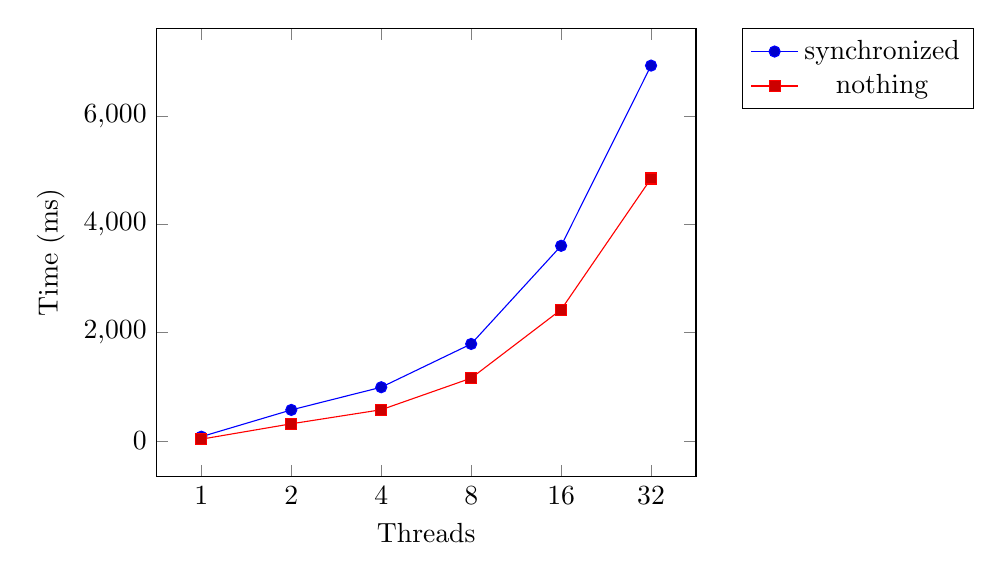
\begin{tikzpicture}
    \begin{axis}[
%      ybar,
      symbolic x coords={1,2,4,8,16,32},
      xtick=data,
      xlabel={Threads},
      ylabel={Time (ms)},
      legend style={at={(1.3,1)},anchor=north}
      ]
      \addplot coordinates {(1,77.39) (2,571.42) (4,990.07) (8,1789.19) (16,3600.88) (32,6927.95)};
      \addplot coordinates {(1,31.37) (2,315.02) (4,574.63) (8,1157.99) (16,2422.88) (32,4843.27)};
      \legend{synchronized, nothing}
    \end{axis}
  \end{tikzpicture}
  \end{center}
\end{frame}

\begin{frame}[fragile]
  \frametitle{Spinlocks, the truth}
    \begin{itemize}
  \item[\faBook]<1-> Do spinlocks just suck then?!
  \item[\faBook]<2-> No not really, they are useful in certain cases, and see a lot of use
    in kernels and RTOS.
  \item[\faBook]<3-> Even the JVM uses it (see e.g. page 232 in the book)!
  \end{itemize}
  \vspace{0.6cm}
  \begin{block}<4->{\faPuzzlePiece \quad Challege time!}
    Can someone come up with a multi-threaded/concurrency situation/problem setting
    where spinlocking, under circumstances, performs consistently and visibly
    better than \texttt{synchronized}? First three to demonstrate win half a point!
  \end{block}
\end{frame}

\section{Latches (and task delegation)}

\begin{frame}[fragile]
  \frametitle{The Problem — Coordinating Threads}
  \begin{block}<1->{\faPuzzlePiece \quad The problem}
    You launch multiple threads to do some work... But how do you wait for all
    of them to finish before moving on?
  \end{block}

  For instance:
  \begin{itemize}
  \item[\faBook]<1-> Wait for all chefs to finish prep before serving.
  \item[\faBook]<1-> Wait for multiple services to initialize before starting the server.
  \item[\faBook]<1-> Wait for data loading to finish before processing.
  \item[\faBook]<1-> Wait for other threads to calculate a number, then perform
    an operation on their results.
  \end{itemize}
\end{frame}

\begin{frame}[fragile]
  \frametitle{Introducing \texttt{CountDownLatch}}
  \begin{block}<1->{\faLightbulb \quad Key idea}
    A \texttt{CountDownLatch} lets one or more threads wait until a set of operations are completed.
  \end{block}

  \vspace{0.4cm}
  \begin{itemize}
  \item[\faBook]<1-> Threads call \texttt{latch.countDown()} when they’re done.
  \item[\faBook]<1-> Main thread calls \texttt{latch.await()} to wait.
  \end{itemize}
\end{frame}

\begin{frame}[fragile]
  \frametitle{\texttt{CountDownLatch} in the code}

\begin{lstlisting}[language = Java , frame = trBL , firstnumber = last ,
escapeinside={(*@}{@*)}]
CountDownLatch latch = new CountDownLatch(NUM); // We expect NUM threads to finish
[...]
for (int i = 0; i < NUM; i++) {
    new Thread(() -> {
        doWork();
        latch.countDown(); // Signal task completion
    }).start();
}
[...]
latch.await(); // Blocks until count == 0
\end{lstlisting}

  \begin{block}<2->{\faExclamationTriangle \quad Important}
    Don't forget to call \texttt{latch.CountDown()} when the thread is done!
  \end{block}
\end{frame}

% Benchmarks done on my (faster) PC, with 16 cores
% 134217728 = 2^27
% 1073741824 = 2^30
% Benchmark: GlobalCounter
% Global     &  1 & 134217728 & 142.63 ms \
% Global     &  1 & 1073741824 & 1091.88 ms \
% Global     &  2 & 134217728 & 683.49 ms \
% Global     &  2 & 1073741824 & 5537.15 ms \
% Global     &  4 & 134217728 & 782.39 ms \
% Global     &  4 & 1073741824 & 6129.00 ms \
% Global     &  8 & 134217728 & 485.40 ms \
% Global     &  8 & 1073741824 & 3899.85 ms \
% Global     & 16 & 134217728 & 465.10 ms \
% Global     & 16 & 1073741824 & 3720.81 ms \
% Global     & 32 & 134217728 & 456.63 ms \
% Global     & 32 & 1073741824 & 3682.52 ms \

% Benchmark: LocalCounter+Latch
% Local+Latch &  1 & 134217728 & 1.32 ms \
% Local+Latch &  1 & 1073741824 & 0.20 ms \
% Local+Latch &  2 & 134217728 & 0.33 ms \
% Local+Latch &  2 & 1073741824 & 0.36 ms \
% Local+Latch &  4 & 134217728 & 0.65 ms \
% Local+Latch &  4 & 1073741824 & 0.59 ms \
% Local+Latch &  8 & 134217728 & 1.15 ms \
% Local+Latch &  8 & 1073741824 & 1.18 ms \
% Local+Latch & 16 & 134217728 & 2.44 ms \
% Local+Latch & 16 & 1073741824 & 2.86 ms \
% Local+Latch & 32 & 134217728 & 5.47 ms \
% Local+Latch & 32 & 1073741824 & 4.74 ms \

% I think in the 2nd, optimized batch the latch really adds noticeable overhead.

\begin{frame}[fragile]
  \frametitle{\texttt{synchronized} vs Latch and delegation ($2^{27}$ increments)}

  \begin{center}
    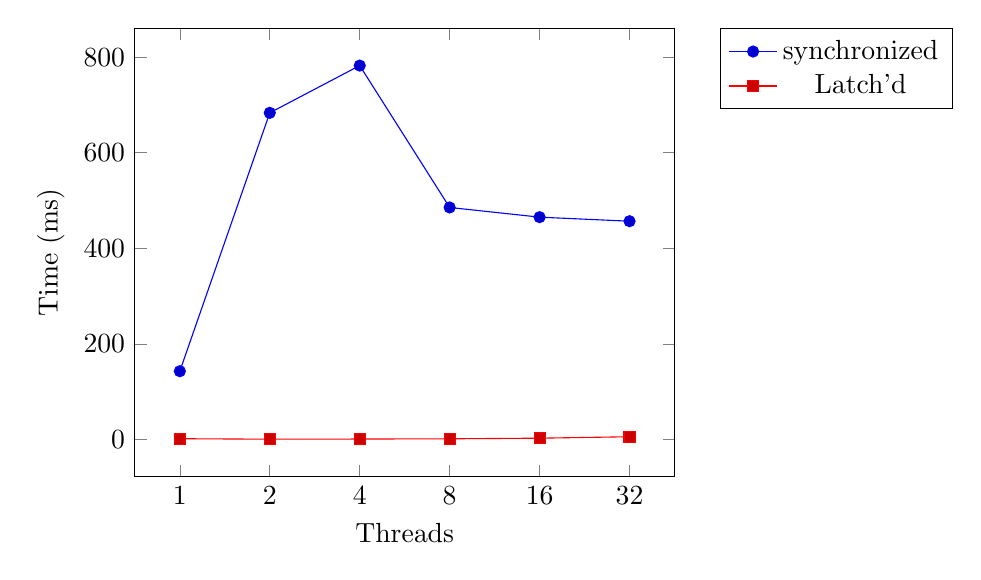
\begin{tikzpicture}
      \begin{axis}[
        % ybar,
        symbolic x coords={1,2,4,8,16,32},
        xtick=data,
        xlabel={Threads},
        ylabel={Time (ms)},
        legend style={at={(1.3,1)},anchor=north}
        ]
        \addplot coordinates {(1,142.63) (2,683.49) (4,782.39) (8,485.40) (16,465.10) (32,456.63)};
        \addplot coordinates {(1,1.32) (2,0.33) (4,0.65) (8,1.15) (16,2.44) (32,5.47)};
        \legend{synchronized, Latch'd}
      \end{axis}
    \end{tikzpicture}
  \end{center}
\end{frame}

\begin{frame}[fragile]
  \frametitle{\texttt{synchronized} vs Latch and delegation ($2^{30}$ increments)}

  \begin{center}
    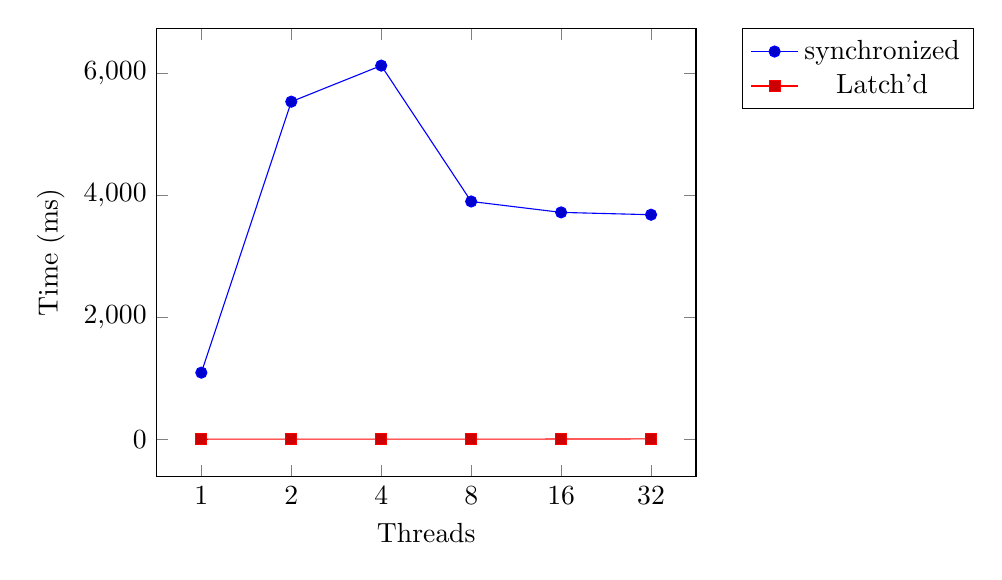
\begin{tikzpicture}
      \begin{axis}[
        % ybar,
        symbolic x coords={1,2,4,8,16,32},
        xtick=data,
        xlabel={Threads},
        ylabel={Time (ms)},
        legend style={at={(1.3,1)},anchor=north}
        ]
        \addplot coordinates {(1,1091.88) (2,5537.15) (4,6129.00) (8,3899.85) (16,3720.81) (32,3682.52)};
        \addplot coordinates {(1,0.20) (2,0.36) (4,0.59) (8,1.18) (16,2.86) (32,4.74)};
        \legend{synchronized, Latch'd}
      \end{axis}
    \end{tikzpicture}
  \end{center}
\end{frame}

% Benchmarks done on my (faster) PC, with 16 core
% Local+Latch &  1 & 137438953472 & 1861.63 ms \
% Local+Latch &  2 & 137438953472 & 949.02 ms \
% Local+Latch &  4 & 137438953472 & 479.90 ms \
% Local+Latch &  8 & 137438953472 & 241.49 ms \
% Local+Latch & 16 & 137438953472 & 200.02 ms \
% Local+Latch & 32 & 137438953472 & 138.73 ms \
% Local+Latch & 64 & 137438953472 & 150.83 ms \

% Local+Latch &  1 & 274877906944 & 3718.28 ms \
% Local+Latch &  2 & 274877906944 & 1885.63 ms \
% Local+Latch &  4 & 274877906944 & 1035.00 ms \
% Local+Latch &  8 & 274877906944 & 486.03 ms \
% Local+Latch & 16 & 274877906944 & 414.80 ms \
% Local+Latch & 32 & 274877906944 & 267.12 ms \
% Local+Latch & 64 & 274877906944 & 304.39 ms \



\begin{frame}[fragile]
  \frametitle{Comparing increments (latch'd): $2^{37}$ vs $2^{38}$}

  \begin{center}
    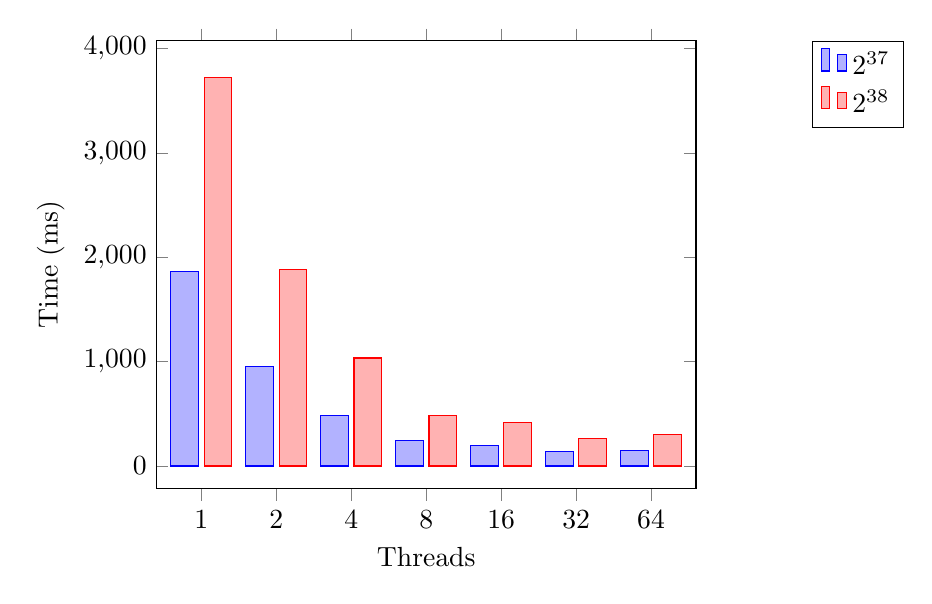
\begin{tikzpicture}
      \begin{axis}[
        ybar,
        symbolic x coords={1,2,4,8,16,32,64},
        xtick=data,
        xlabel={Threads},
        ylabel={Time (ms)},
        legend style={at={(1.3,1)},anchor=north}
        ]
        \addplot coordinates {(1,1861.63) (2,949.02) (4,479.90) (8,241.49) (16,200.02) (32,138.73) (64,150.83)};
        \addplot coordinates {(1,3718.28) (2,1885.63) (4,1035.00) (8,486.03) (16,414.80) (32,267.12) (64,304.39)};
        \legend{$2^{37}$,$2^{38}$}
      \end{axis}
    \end{tikzpicture}
  \end{center}
\end{frame}

\begin{frame}[fragile]
  \frametitle{Summarizing latches}

  \begin{itemize}
  \item[\faBook]<1-> Great for coarse, one-shot coordination.
  \item[\faBook]<1-> Very simple, with \texttt{await()} and \texttt{countDown()}.
  \item[\faBook]<1-> Use it to block until (all or some) other threads signal
    they’re done.
    \begin{itemize}
      \item[\faCheck] One does not need to carry \emph{references} of the
        threads around the code.
      \item[\faWindowClose] Can only do this one thing.
    \end{itemize}
  \item[\faBook]<2-> For reusability or bidirectional sync, look into
    \texttt{CyclicBarrier} or \texttt{Phaser}.
  \end{itemize}

\end{frame}

\begin{frame}[fragile]
  \frametitle{Efficient concurrent programming}

  \begin{itemize}
  \item[\faUserInjured]<1-> Blocking (and thus blocking locks) greatly hurts
    performance.
  \item[\faBook]<1-> Generally, thread-safety primitives incur significant
    overhead.
  \item[\faBook]<1-> Thus, performance and thread-safety are competing against
    each other.
  \item[\faBook]<1-> It is up to the programmer to find the right balance, via
    correct design and solid command of the invariants.
  \end{itemize}

  \vspace{0.4cm}
  \begin{block}<2->{\faLightbulb \quad Key idea}
    In order to avoid blocking, one should synchronize as \textbf{little} as
    \textbf{possible}.
    Assigning to each thread independent tasks is \textbf{crucial}.
  \end{block}
\end{frame}

\section{Concurrent Collections}

\begin{frame}[fragile]
  \frametitle{Delegating thread safety}

  \begin{block}<1->{\faBook \quad Delegation}
    Using an object's inherent synchronization capabilities to ensure thread-safety.
  \end{block}

  \vspace{0.4cm}
  \begin{itemize}
  \item[\faBook]<2-> Classes such as \texttt{AtomicInteger}, \texttt{AtomicLong},
    \texttt{AtomicBoolean} offer thread-safe primitive variables.
  \item[\faBook]<3-> Classes such as \texttt{SynchronizedList} and
    \texttt{SynchronizedMap} offer thread-safe \emph{collections}.
  \item[\faBook]<4-> \emph{Concurrent collections} are also another (largely)
    thread-safe collection of Java \emph{collections}.
  \end{itemize}
\end{frame}

\begin{frame}[fragile]
  \frametitle{\texttt{synchronizedMap()} vs \texttt{ConcurrentHashMap}}

  \begin{table}[h]
\centering
\begin{tabularx}{\textwidth}{|l|X|X|}
\hline
\textbf{Aspect} & \texttt{synchronizedMap} & \texttt{ConcurrentHashMap} \\
\hline
Thread safety & Each method synchronized & Fully thread-safe \\
\hline
Granularity & One lock for all ops & Per-element (bucket) or lock-free \\
\hline
Performance under load & Low: lots of contention & High scalability \\
\hline
Compound operations & Manually synchronized & \texttt{putIfAbsent},
\texttt{compute}, \texttt{merge} are atomic\\
\hline
Iteration safety & Must externally synchronize & Safe to iterate \\
\hline
Allows \texttt{null} & Keys and values allowed & \textbf{No} Null keys/values  \\
\hline
Implementation & Wrapper around regular \texttt{Map} with \texttt{synchronized}
& Custom concurrent structure, element-level locks\\
\hline
\end{tabularx}
\caption{Comparison of \texttt{Collections.synchronizedMap()} and \texttt{ConcurrentHashMap}}
\end{table}
\end{frame}

\begin{frame}[fragile]
  \frametitle{Code Listings}

  \begin{itemize}
  \item[\faCode]<1-> LockTestHarness/Spinlock.java: Spinlock implementation
  \item[\faCode]<1-> LockTestHarness/LockTestHarness.java: Spinlock vs
    \texttt{synchronized} (single-run)
  \item[\faCode]<1-> LockTestHarness/LockTestHarness2.java: Spinlock vs
    \texttt{synchronized} (benchmark)
  \item[\faCode]<1-> LatchTestHarness/LatchTestHarness.java: Latch (local
    updates) vs
    \texttt{synchronized} (single)
  \item[\faCode]<1-> LatchTestHarness/LatchTestHarness2.java: Latch (local
    updates) vs
    \texttt{synchronized} (benchmark)
  \item[\faCode]<1-> LatchTestHarness/LatchTestHarness2Long.java: Proper
    benchmarking for latching and local updates using \texttt{long}'s.
  \item[\faCode]<1-> LatchTestHarness/LatchTestHarness2LongMap.java: Latch
    (local updates) vs \texttt{ConcurrentHashMap}.
  \end{itemize}

\end{frame}

\begin{frame}{}
  \centering \huge
  Thank you!
\end{frame}

\end{document}

%%% Local Variables:
%%% mode: latex
%%% TeX-engine: xetex
%%% TeX-master: t
%%% End:
